\documentclass[10.5pt,a4paper]{article}
\usepackage[a4paper,margin=2.2cm,top=2.3cm,bottom=2.4cm]{geometry}
\usepackage{fontspec}
\usepackage{unicode-math}
\setmainfont{TeX Gyre Pagella}
\setsansfont{Inter}[Scale=0.88]
\setmonofont{DejaVu Sans Mono}[Scale=0.80]
\setmathfont{DejaVu Math TeX Gyre}[Scale=0.95]
\usepackage{microtype}
\usepackage{xcolor}
\definecolor{accent}{HTML}{1F4E79}
\definecolor{muted}{HTML}{5F6670}
\definecolor{codebg}{HTML}{F6F7F9}
\definecolor{rule}{HTML}{D9DCE1}
\usepackage{graphicx}
\usepackage{booktabs,tabularx,array}
\usepackage{enumitem}
\setlist{nosep,leftmargin=1.4em,topsep=3pt}
\usepackage[font=small,labelfont={bf,sf},labelsep=period,skip=4pt]{caption}
\usepackage{titlesec}
\titleformat{\section}{\sffamily\large\bfseries\color{accent}}{\thesection}{0.7em}{}
\titleformat{\subsection}{\sffamily\normalsize\bfseries}{\thesubsection}{0.6em}{}
\titleformat{\subsubsection}[runin]{\sffamily\small\bfseries}{}{0em}{}[.]
\titlespacing*{\section}{0pt}{14pt}{6pt}
\titlespacing*{\subsection}{0pt}{10pt}{4pt}
\usepackage{fancyhdr}
\pagestyle{fancy}\fancyhf{}
\renewcommand{\headrulewidth}{0.4pt}
\renewcommand{\headrule}{\hbox to\headwidth{\color{rule}\leaders\hrule height \headrulewidth\hfill}}
\fancyhead[L]{\sffamily\footnotesize\color{muted}\ReportShortTitle}
\fancyhead[R]{\sffamily\footnotesize\color{muted}S. K. Eshraghi Naeini}
\fancyfoot[C]{\sffamily\footnotesize\color{muted}\thepage}
\usepackage{listings}
\lstdefinelanguage{VerilogX}[]{Verilog}{morekeywords={localparam,integer,genvar,generate,endgenerate}}
\lstset{language=VerilogX,basicstyle=\ttfamily\footnotesize,keywordstyle=\color{accent}\bfseries,
  commentstyle=\color{muted}\itshape,stringstyle=\color{teal!70!black},numbers=left,numberstyle=\tiny\color{muted},
  numbersep=6pt,backgroundcolor=\color{codebg},frame=single,rulecolor=\color{rule},framesep=4pt,
  xleftmargin=14pt,breaklines=true,columns=fullflexible,keepspaces=true,showstringspaces=false,
  tabsize=4,aboveskip=6pt,belowskip=6pt}
\usepackage{tikz}
\usetikzlibrary{arrows.meta,positioning,shapes.geometric,calc,fit,automata}
\tikzset{blk/.style={draw=accent,thick,fill=accent!6,rounded corners=2pt,minimum height=8mm,minimum width=20mm,align=center,font=\sffamily\small},
         io/.style={font=\sffamily\footnotesize,align=center},
         arr/.style={-{Stealth[length=2mm]},semithick},
         st/.style={state,draw=accent,thick,fill=accent!6,minimum size=9mm,font=\sffamily\footnotesize,inner sep=1pt,align=center}}
\usepackage{xurl}
\usepackage[colorlinks=true,linkcolor=accent,urlcolor=accent,citecolor=accent]{hyperref}
\usepackage{siunitx}
\sisetup{group-separator={,},group-minimum-digits=4}
\newcommand{\sig}[1]{\texttt{#1}}
\newcommand{\pass}{\textcolor{green!45!black}{\textsf{\textbf{PASS}}}}
\newcommand{\repo}{https://github.com/seyedkiarash/seyedkiarash.github.io/tree/main/labs/logic-circuits-lab}
\newcommand{\note}[1]{\par\smallskip\noindent\colorbox{accent!7}{\parbox{\dimexpr\linewidth-2\fboxsep}{\small #1}}\par\smallskip}
\setlength{\parindent}{0pt}
\setlength{\parskip}{4pt}

\newcommand{\ReportTitle}[3]{%
  \thispagestyle{plain}
  {\sffamily\small\color{muted}Logic Circuits Laboratory \textbullet\ Department of Electrical Engineering, Sharif University of Technology\par}
  \vspace{2pt}
  {\sffamily\LARGE\bfseries #1\par}
  \vspace{1pt}
  {\sffamily\Large #2\par}
  \vspace{6pt}
  {\color{rule}\hrule height 0.6pt}
  \vspace{5pt}
  {\small
  \begin{tabular}{@{}l@{\hspace{2em}}l@{}}
    \textcolor{muted}{Student}  & Seyed Kiarash Eshraghi Naeini (403101383)\\
    \textcolor{muted}{Instructor} & Dr.\ Mohammad Reza Movahhedin \quad\textcolor{muted}{Teaching assistant:} Hossein Moghim\\
    \textcolor{muted}{Semester} & Fall 2025 \quad\textcolor{muted}{session:} #3\\
    \textcolor{muted}{Platform} & Zynq-7010 (XC7Z010-CLG400-1), \SI{50}{MHz} clock, Vivado 2019.1
  \end{tabular}\par}
  \vspace{4pt}
  {\color{rule}\hrule height 0.6pt}
  \vspace{8pt}}

\newcommand{\ReportShortTitle}{Midterm experiment -- Decoders, BCD addition, comparators and multiplexers}
\begin{document}
\ReportTitle{Midterm Experiment}{Decoders, BCD Addition, Comparators, Multiplexers and a Multiplier}{7--8 December 2025}

\section*{Summary}
This midterm experiment (between Experiments 4 and 6) implements a set of standard combinational building blocks on the FPGA: a 3-to-8
decoder, a one-digit BCD adder with input validation, 4-bit magnitude comparators (once behaviourally and
once from the status flags of a subtractor), an 8-to-1 multiplexer and a $4\times4$ multiplier. Because all
designs have at most eight inputs, each was verified \emph{exhaustively} for this report. This found one
error in the flag-based signed comparator (28 of 256 input pairs) and two wiring errors in the second
bonus design; all are analysed and corrected below, and the bonus now works as a 2-bit comparator.
Code: \url{\repo/lab04m-midterm-decoders-comparators}.

Inputs and outputs follow the extension board: the operands are \sig{A = DIP[3:0]} and
\sig{B = DIP[7:4]}; results appear on \sig{LED[9:0]} and the seven-segment display; the four board push
buttons are \emph{active-low} and are inverted in the designs.

\section{Part 1 -- 3-to-8 decoder}
Each output is the minterm of the 3-bit input, e.g.\ $\text{show}_5 = n_2\,\overline{n_1}\,n_0$, so exactly
one of \sig{LED[7:0]} is lit -- the one selected by \sig{DIP[2:0]}. Exhaustive test: all 256 DIP settings
give the correct one-hot output.

\section{Part 2 -- BCD adder}
\subsection{Design}
The two digits are added by a 4-bit ripple-carry adder (four full adders built from half adders). The
binary sum $S$ (0--18) is then converted to BCD:
\begin{itemize}
  \item if the adder produced a carry ($S\geq16$): tens $=1$, units $=(16+S_{3:0})-10$;
  \item else if $S\geq10$: tens $=1$, units $=S-10$;
  \item otherwise tens $=0$, units $=S$.
\end{itemize}
Subtracting 10 from a 5-bit value is equivalent to the familiar ``add 6 and drop the carry'' correction.
A helper \sig{check10} flags operands that are not BCD digits, $A\geq10 \iff A_3(A_2+A_1)$; an invalid
input shows \texttt{E}, and if both are invalid a second digit shows \texttt{E} as well. The units digit is
shown on the display and the tens on \sig{LED[0]} (Fig.~\ref{fig:bcd}).
\begin{figure}[h]
\centering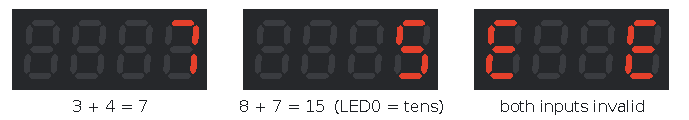
\includegraphics[width=0.62\linewidth]{figures/midterm_bcd.pdf}
\caption{BCD adder output for three inputs.}\label{fig:bcd}
\end{figure}

\subsection{Verification}
All 256 input pairs: the 100 valid digit pairs give the correct units digit and tens LED, and the 156
pairs with an invalid digit show \texttt{E} on one or two digits as specified. 0 errors.

\section{Part 3 -- 4-bit comparators}
Three outputs are produced: $A>B$ unsigned (\sig{LED[0]}), $A>B$ signed in two's complement
(\sig{LED[1]}) and $A=B$ (\sig{LED[2]}).

\subsection{3a -- Behavioural description}
The unsigned and equality tests use the Verilog operators. The signed test first compares the sign
bits -- if they differ, the non-negative operand is larger -- and otherwise compares the remaining three
bits, which order two's-complement numbers of equal sign correctly. All 256 pairs: 0 errors.

\subsection{3b -- Comparison from subtractor flags}
The second version computes $A-B = A+\overline{B}+1$ with the adder and derives the comparisons from the
flags $Z$ (zero), $C$ (carry, i.e.\ no borrow), $N$ (sign of the result) and $V$ (overflow):
\[
A>B\ \text{(unsigned)} = C\,\overline{Z}, \qquad
A>B\ \text{(signed)} = \overline{Z}\,\overline{(N\oplus V)}, \qquad
A=B = Z .
\]
\textbf{Finding.} The submitted design computed $V$ with the overflow formula of an \emph{addition}
of $A$ and $B$, $V=A_3B_3\overline{S_3}+\overline{A_3}\,\overline{B_3}S_3$, although the adder actually adds
$A$ and $\overline{B}$. Its signed output was also built from a different expression,
\[
N\,\overline{(N\oplus V)}\,\overline{V} \;+\; \overline{N}\,C\,\overline{Z} \;+\; \overline{A_3}\,B_3 ,
\]
whose first term is always 0. Exhaustive simulation of the submitted code gave the wrong answer for
\textbf{28 of the 256} pairs -- exactly the pairs with $A<0<B$ whose difference underflows, $A-B<-8$
(e.g.\ $A=-8$, $B=1$ was reported as ``greater''). The corrected design uses the subtraction overflow
$V=A_3\overline{B_3}\,\overline{S_3}+\overline{A_3}B_3S_3$ and the standard condition above; it now matches
the behavioural comparator on all 256 pairs.

\section{Part 4 -- 8-to-1 multiplexer}
The DIP switches are the eight data inputs and the inverted buttons \sig{button[2:0]} the select code;
the selected bit is shown on \sig{LED[0]}. The submitted version described the selection with a chain of
\texttt{if}\ldots\texttt{else if} statements; it is written here as \sig{assign f = A[s]}, which is
equivalent and cannot infer a latch. Exhaustive test: 256 data words $\times$ 8 select codes, 0 errors.

\section{Bonus 1 -- \texorpdfstring{$4\times4$}{4x4} combinational multiplier}
The product is formed by shift-and-add: for every bit $B_i=1$ the partial product $A\cdot2^i$ is added,
$P=\sum_i B_i\,(A\ll i)$, giving an 8-bit result (maximum $15\times15=225$) on \sig{LED[7:0]}. All 256
products are correct. Synthesis maps the four conditional additions to 23 LUTs and carry logic.

\section{Bonus 2 -- A 2-bit comparator from multiplexers}
\subsection{Idea}
The bonus builds a comparator for two 2-bit numbers $X=\{x_1,x_0\}$ and $Y=\{y_1,y_0\}$ (from the
inverted buttons: $x_0=n_0$, $y_0=n_1$, $x_1=n_2$, $y_1=n_3$) using \emph{only} 8-to-1 multiplexers, each
used as a three-input look-up table: the constant on the data inputs is the truth table and the three
signals on the select inputs are the variables. As in Part 3b the comparison is done by subtraction
$X-Y$:
\begin{itemize}
  \item two multiplexers with the table \texttt{1001\,0110} (three-input XOR) give the difference bits
        $d_0 = x_0\oplus y_0$ and $d_1 = x_1\oplus y_1\oplus b_0$;
  \item two multiplexers with the table of the \emph{borrow} function,
        $b_\text{out} = \overline{x}\,y + \overline{(x\oplus y)}\,b_\text{in}$, i.e.\ \texttt{1000\,1110}
        for select $\{x,y,b_\text{in}\}$, give the borrow chain $b_0$ and $b_1$;
  \item $X<Y = b_1$, \quad $X=Y = \overline{d_0}\,\overline{d_1}$, \quad $X\geq Y = \overline{b_1}$.
\end{itemize}

\subsection{Findings in the submitted version and correction}
\begin{itemize}
  \item The select buses of the borrow multiplexers were declared without a width,
        \texttt{wire s1 = \{nb[2], nb[0], Cin\};}, which in Verilog declares a \emph{1-bit} wire: only the last
        element survived, so the borrow chain (and \sig{LED[0]}) did not depend on the buttons at all.
  \item The borrow multiplexers paired the operand bits as $(n_2,n_0)$ and $(n_3,n_1)$, whereas the XOR
        multiplexers paired them as $(n_0,n_1)$ and $(n_2,n_3)$. An exhaustive search over all 256
        possible tables showed that no table makes this wiring a comparator.
  \item The borrow table was taken from the DIP switches. With the pairing corrected, exactly one
        setting works -- \texttt{1000\,1110}, the borrow function above -- which confirms the intended design.
\end{itemize}
The corrected design declares the select buses as 3-bit vectors, uses the same bit pairing in both
chains and stores the borrow table as a constant, so it works without a particular DIP setting.
Exhaustive test: all 16 operand pairs give the correct $\geq$, $=$, $<$ outputs (checked for 16 different
DIP settings to confirm the DIP switches no longer matter).

\section{Implementation results}
\begin{table}[h]
\centering\small
\caption{Resources after synthesis (Yosys, Xilinx 7-series mapping).}
\begin{tabular}{@{}lrl@{}}
\toprule
Design & LUTs & Note\\
\midrule
Part 1 -- 3-to-8 decoder & 8 & \\
Part 2 -- BCD adder & 20 & \\
Part 3a / 3b -- comparators & 10 / 10 & \\
Part 4 -- 8-to-1 multiplexer & 3 & \\
Bonus 1 -- multiplier & 23 & \\
Bonus 2 -- 2-bit comparator & 3 & one LUT per output\\
\bottomrule
\end{tabular}
\end{table}

\section{Verification summary}
\begin{table}[h]
\centering\small
\begin{tabularx}{\linewidth}{@{}lXr@{}}
\toprule
Testbench & What is checked (exhaustive) & Result\\
\midrule
\sig{tb\_part1} & 256 DIP settings, one-hot output & \pass\\
\sig{tb\_part2} & 100 valid digit pairs, 156 invalid inputs & \pass\\
\sig{tb\_part3} & 256 pairs $\times$ 3 comparisons & \pass\\
\sig{tb\_part52} & 256 pairs $\times$ 3 comparisons (corrected flags) & \pass\\
\sig{tb\_part4} & 256 data words $\times$ 8 select codes & \pass\\
\sig{tb\_multiplier} & all 256 products & \pass\\
\sig{tb\_bonus2} & all 16 operand pairs, $\geq$ / $=$ / $<$ & \pass\\
\bottomrule
\end{tabularx}
\end{table}

\section{Conclusion}
The standard combinational blocks map to a handful of LUTs each. Comparing two implementations of the
same function -- behavioural and flag-based -- and testing them exhaustively was decisive: the flag-based
signed comparison is correct only with the overflow flag of the operation actually performed, and the
only failing inputs were the 28 overflow cases. The bonus shows that multiplexers used as look-up
tables can build any logic function, and how an undeclared vector width silently changes a circuit.

\end{document}
